\documentclass[10pt, a4paper, titlepage]{article}

% font size could be 10pt (default), 11pt or 12 pt
% paper size coulde be letterpaper (default), legalpaper, executivepaper,
% a4paper, a5paper or b5paper
% side coulde be oneside (default) or twoside 
% columns coulde be onecolumn (default) or twocolumn
% graphics coulde be final (default) or draft 
%
% titlepage coulde be notitlepage (default) or titlepage which 
% makes an extra page for title 
% 
% paper alignment coulde be portrait (default) or landscape 
%
% equations coulde be 
%   default number of the equation on the rigth and equation centered 
%   leqno number on the left and equation centered 
%   fleqn number on the rigth and  equation on the left side
%	

\usepackage{colortbl}
\usepackage{graphicx}
\usepackage{kotex}
\usepackage{authblk}
\usepackage{amsmath}
\usepackage{textcomp}
\usepackage{array}
\usepackage[labelfont=bf]{caption}
\usepackage{subcaption}
\usepackage{longtable}

\DeclareGraphicsExtensions{.png}

%\title{A not so small \LaTeX{} Article Template\thanks{To your mother} 그렇습니다.}
\title{
	Programming Language Propagation in GitHub
}
\author[ ]{김슬기\thanks{seulgi.kim@snu.ac.kr}}
\author[ ]{김찬민\thanks{kcm1700@snu.ac.kr}}
\author[ ]{황호성\thanks{thefron@snu.ac.kr}}
\affil[ ]{서울대학교 컴퓨터공학부}

\date{\today} 
% \date{\today} date coulde be today 
% \date{25.12.00} or be a certain date
% \date{ } or there is no date 
\begin{document}
% Hint: \title{what ever}, \author{who care} and \date{when ever} could stand 
% before or after the \begin{document} command 
% BUT the \maketitle command MUST come AFTER the \begin{document} command! 
\maketitle


\begin{abstract}
현대의 성공적인 소프트웨어 개발은 보통 개인의 힘으로 이루어지지 않는다. 커뮤니티에서 영향력이 있는 소프트웨어는 여러 사람의 협업에 의해서 발전해 나간다. 그리고 이러한 협업 과정 속에서 개발자들은 서로에게 영향을 받는다. 그리고 그 영향에는 당연히 소프트웨어 개발의 핵심적인 매개 중 하나인 프로그래밍 언어도 포함된다. 이 연구에서는 오픈 소스 소프트웨어 커뮤니티인 GitHub을 분석해 개발자 간 네트워크와 프로그래밍 언어 전파 사이의 상관 관계를  조사하였다.

우선 어떤 개발자가 특정 프로그래밍 언어를 새로이 사용하게 되는 이유에 social influence가 작용을 하는지 여부를 확인하기 위해 GitHub의 개발자 네트워크와 그들이 사용하는 프로그래밍 언어 사이에서 세 가지 대표적인 closure, 즉 (i)triadic closure, (ii)focal closure, (iii)membership closure가 생성되는 양상을 각각 분석하였다. 다양한 소셜 네트워크에서 관찰된 것처럼 관계가 있는 공통된 개발자가 많을수록 관계가 생길 확률이 높았고, 공통된 언어 집합이 클수록 관계가 생길 확률이 높았다. 언어마다 관계가 생성되는 양상이 달랐다.


그리고 우리는 전통적으로 많이 쓰이는 프로그래밍 언어와 새롭게 개발돼 개발자들 사이에서 입소문을 타고 전파되는 프로그래밍 언어의 전파 양상에는 차이가 있을 것을 가정하고, 개발자가 새로운 프로그래밍 언어를 쓰기 시작하는 시점에 얼마나 많은 지인들이 해당 언어를 쓰고 있는지를 시간에 따른 weakly connected component의 변화를 통해 분석하였다. 그 결과, 예상한 것처럼 전통적으로 시스템 개발에 쓰여온 언어들을 사용하는 것은 개발자들 사이의 관계에 영향을 덜 받는다는 사실을 알 수 있었다.
\\ \\
{\bf Keywords}: GitHub, Programming Language, Propagation, Social Network, Information Diffusion
\end{abstract}

\tableofcontents % create a table of contens 

\newpage


\section{서론}
현대의 개발은 단독으로 이루어지지 않는다. 대부분의 영향력있는 소프트웨어는 여러 사람의 협업에 의해서 개발되는 과정에서 다듬어지고 성숙해 나간다. 지금까지 이러한 소프트웨어 개발 협업을 위해 수많은 플랫폼이 나왔다. 현재 가장 대표적인 플랫폼으로 GitHub을 들 수 있다. GitHub은 2008년부터 서비스를 시작한 오픈 소스 소프트웨어 커뮤니티다\cite{r1}.
서비스 공개 이후 빠른 속도로 성장하였고, 현재는 오픈 소스 소프트웨어 호스팅 서비스 중 가장 큰 서비스가 되었다. GitHub은 기존의 오픈 소스 커뮤니티와 달리 소셜 코딩을 표방해 개발자 사이의 네트워킹을 강조한 덕에 협업으로 진행되던 수많은 유명한 프로젝트들이 GitHub으로 옮겨오게 되었고, 그 성장세가 급격히 커져 현재 가장 큰 오픈 소스 소프트웨어 커뮤니티로 자리매김하고 있다.


트위터, 페이스북 등 일반적인 소셜 네트워크 서비스(SNS)에서는 개발자 간의 기존 관계나 관심 주제 등을 기반으로 네트워크가 형성된다. GitHub은 이러한 전략을 채택해 개발자 간의 네트워크 형성을 독려하고 상호 간의 활동 기록을 보여줌으로써 개발자들을 같은 프로젝트에 기여하게 하기도 하고 프로젝트가 유명해지도록 돕거나 나아가 특정 프로젝트에 관심 있는 사람들이 해당 프로젝트에 사용된 언어를 새로이 사용하도록 만들기도 한다. 우리는 여기서 착안해 GitHub 개발자들의 팔로우 그래프를 이용해 지인 네트워크가 프로그래밍 언어 전파에 미치는 영향을 연구해 보았다.


우리는 우선 GitHub의 네트워크 구조가 어떻게 되었는지를 조사하였다. 이를 위해 개발자간의 관계, 개발자와 언어 사이의 관계, 언어간의 관계를 조사하였다. 개발자간의 관계를 이해하기 위해서 팔로우 그래프의 degree를 계산하였다. 이는 개발자 네트워크의 대략적인 규모를 아는데 도움을 주었다. 개발자와 언어 사이의 관계를 이해하기 위해서 여러 언어를 사용하는 개발자가 얼마나 있는지 조사하였다. 이를 통하여 대부분의 개발자들이 사용하던 언어를 고수하는 것이 아닌 상황에 맞게 다양한 언어를 사용한다는 것을 알 수 있었다. 또한, 언어별로 여러 언어를 사용할 수 있는 개발자의 비율을 조사하여, PHP, C\#, Java, JavaScript 등과 같이 전통적인 언어일수록 한 가지 언어를 사용하는 개발자의 비율이 높지만, C는 예외라는 것을 보았다. 마지막으로 언어 사이의 관계를 알기 위하여, 언어를 사용하는 집단 사이의 관계를 보았다. 가장 많은 개발자를 공유하는 언어집단은 무엇인지도 보았다. 이를 통하여 GitHub의 개발자는 웹개발을 하는 사람이 대부분이라는 것을 알 수 있었다. 또한, 언어별 개발자 집단 사이의 Jaccard Distance를 계산하였다. 이를 통해 사람들이 새로 습득한 언어의 대부분은 기존에 사용하던 언어와 비슷하거나 같이 사용했을 때 도움이 되는 언어를 선택한다는 것을 알 수 있었다. 따라서 이런 연관 관계가 약한 새로운 언어를 사용하기 시작한다면, 이는 언어의 기능 때문이 아니라 다른 요인에 의한 것이라고 볼 수 있다.




D. Easley  2010 \cite{r2}에 의하면 소셜 네트워크에서 Affiliation Network를 구성하면, 관계가 형성되는 과정을 세 가지 관점에서 볼 수 있다. (i)두 사람 사이에 형성된 관계 사이에 공통된 이웃 사람이 있는 경우 triadic closure라고 하고, (ii)두 사람 사이에 형성된 관계 사이에 공통된 foci가 있는 경우 focal closure라고 하고, (iii)사람과 foci 사이에 형성된 관계 사이에 공통된 사람이 있는 경우 membership closure라고 한다. 새로운 프로그래밍 언어를 습득하는 것에 social influnce 효과가 있는지 여부를 확인하기 위해, foci를 프로그래밍 언어로 하여 위 세가지 closure가 생성되는 양상을 연구해 보았다.


마지막으로 우리는 오랜 기간 동안 많이 쓰여왔거나 학습용으로 습득하는 언어의 전파는 social influence보다는 각 개인이 독립적으로 사용하기 시작할 것이고, 상대적으로 최근에 나왔거나 입소문을 타고 퍼지는 언어는 가까운 지인 네트워크의 영향을 크게 받을 것이라 가정하였다. 이를 알아보기 위해 기간에 따라 개발자들이 새로운 언어를 사용하기 시작한 시점을 수집해 특정 개발자와 특정 언어 사이에 링크가 형성될 때 weakly connected component가 얼마나 많이 형성되는 지 분석해 보았다. 전파 과정에서 weakly connected component가 상대적으로 많이 형성되는 언어는 개별적으로 사용하기 시작한 언어, 즉 오랜 기간 쓰여 온 언어이거나 언어 학습 용도로 많이 가르치는 언어일 것이고 새로운 언어의 습득이 strongly connected component에서 이루어진다면 좀 더 주변 지인에 의해 전파되는 특성이 강한, 상대적으로 새로 유행하는 언어일 것으로 판단할 수 있을 것이라 추측하고 연구하였다.


\section{관련 연구}

Meyerovich 2013 \cite{r3}은 개발자들이 사용할 언어를 채택할때 어떤 것이 중요한가를 조사하였다. 하지만 개발자간의 관계가 아닌 언어 자체의 기능과 라이브러리 등을 중심으로 봤다. 우리의 연구는 언어 자체보다는 개발자들 사이의 관계에 주목하였다.


Thung 2013 \cite{r4}은 GitHub의 개발자들 사이에 생기는 네트워크 구조에 대해서 조사하였다. 이 연구에서는 같은 프로젝트에 참여했던 개발자들 사이에 간선을 이어 네트워크를 만들었다. 이로 인해 만들어진 네트워크에서 개발자들 사이의 최대 거리가 그렇게 멀지 않다는 것을 보였다.

Yu 2014 \cite{r5}에서는 개발자들 사이의 팔로우를 이용하여 네트워크를 구성하여, 네트워크에서 생기는 패턴을 분석하였다.


개발자와 언어 사이의 네트워크 구조의 특성을 분석하기 위해 \cite{r2}의 Chapter 4에 나오는 Triadic Closure, Focal Closure, Membershi Closure를 이용하였다.

\section {자료 수집}

GitHub에는 1400만명 이상의 개발자와 200만 개 이상의 프로젝트가 존재한다. 모든 개발자와 프로젝트를 분석할 수도 있지만, 모든 개발자와 프로젝트가 유효한 개발자는 아니다. Antonio Lima 2014 \cite{r6} 연구에 따르면 GitHub에 등록된 프로젝트 중 63\%만이 최소 한 개 이상의 커밋을 가지고 있고, 그 중에서 74\%에 해당하는 프로젝트만이 2명 이상의 기여자가 있다. 개발자 간의 네트워크가 미치는 영향을 연구하는 목적에 부합하기 위해 일정 수준 이상의 활동과 기여자를 가진 프로젝트를 추려낼 필요가 있다. 특히 데이터 수집에 사용한 GitHub API \cite{r7}는 시간당 API 호출 횟수가 5,000 건으로 제한돼 있기 때문에 최대한 유의미한 규모를 가진 프로젝트와 해당 프로젝트의 개발자 정보만 수집할 수 있도록 그 대상을 한정하였다.

	필요한 개발자와 프로젝트만 추출하기 위해서 우리는 GitHub Archive \cite{r8}를  이용했다. GitHub Archive는 GitHub에서 발생한 event \cite{r9} 들을 수집해놓은 사이트이다. Github Archive에서 제공하는 데이터 중 최근 1년 4개월의 event를 분석하여 꾸준한 활동이 있는 개발자와 프로젝트 목록를 추려내었다.


개발자 정보는 2015년 1월부터 2016년 4월까지 16개월동안 연속으로 매달 활동 기록이 있는 개발자를 대상으로 수집하였다. 105,932 명의 개발자가 대상이 되었다. 수집 항목은 following 목록, follower 목록이었다.


프로젝트 정보는 2016년 4월 활동이 있었던 프로젝트를 대상으로 수집하였다. 2,572,202개의 후보가 있었고, 자료 수집 시점인 2016년 5월 20일에 1,911,602개의 프로젝트에 접근할 수 있었다. 수집 항목은 이름, 소유한 개발자, 언어, fork한 개발자 목록, subscribe한 개발자 목록이었다.

개발자 정보는 약 10일 간격으로 3회에 걸쳐 수집하였다. 나중에 설명할 세 가지 타입의 closure 분석에 필요한 자료이다. following / follower 관계가 형성되는 사건은 GitHub Archive에서 확인할 수 없기 때문에 시간에 따른 변화를 보기 위해 스냅숏이 필요했다.	개발자와 프로젝트 사이의 관계 형성은 GitHub Archive의 기록에서 확인할 수 있었다.

개발자마다 언어 사용 정보도 계산했다. 개발자가 사용하는 언어의 범위는 직접 소유한 프로젝트, fork한 프로젝트, subscribe한 프로젝트들의 언어로 하였다.


\begin{table}[ht]
\begin{tabular}{|m{2.5cm}|m{4cm}|m{4.0cm}|}

\hline

종류 & 항목 & 기간 \\

\hline

GitHub Archive Strong Event &
Push, PullRequest 이벤트 &
2015년 1월 $\sim$ 2016년 4월 \\

\hline

GitHub Archive Weak Event &
모든 종류의 이벤트&
2015년 1월 $\sim$ 2016년 4월 \\

\hline

GitHub Repository &
이름, 소유자, 언어, fork한 사용자 목록, subscribe한 사용자 목록 &
2016년 5월 \\

\hline

GitHub User &
following 개발자 목록,
follower 개발자 목록 &
2016년 5월 $\sim$ 6월 (3회)\\

\hline
\end{tabular} 

\caption{
	수집하는 데이터의 종류와 세부 항목. 기간은 데이터가 어떤 기간의 상태를 나타내는지 요약한 것이다.
}
\label{tab:collect}
\end{table}


\section{자료 분석}
\subsection{개발자간의 관계}
먼저 수집한 자료를 기반으로 following과 follower의 degree 분포를 분석해보았다. 2016년 5월 28일 기준 자료이다. 다음 \bf{Figure} \ref{fig:fdist}\rm은 가로 축을 degree로 하고 세로 축을 해당하는 user의 수로 하여 그린 그래프이다. 각 축은 log scale이다. following 그래프에서 power law exponent는 1.90이었고, follower 그래프에서 power law exponent는 1.77이었다. 각각 $R^2$ 값은 0.92, 0.94이다. following의 경우 최대값은 130612이고, follower의 경우 최대값은 38218이었다.


\begin{figure}
	\begin{subfigure}{0.99\textwidth}
		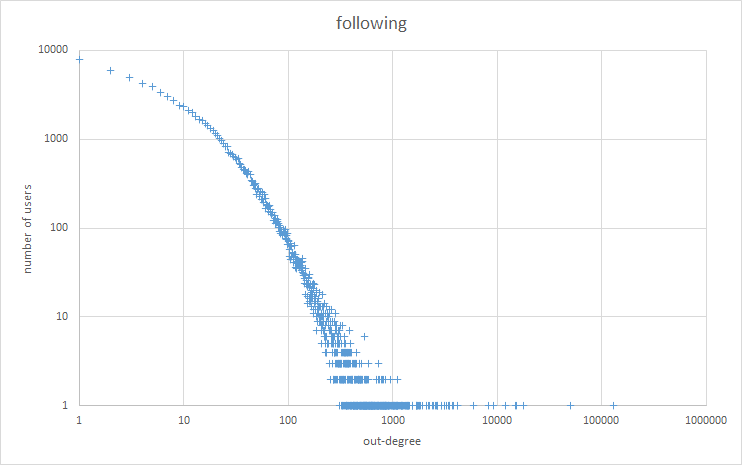
\includegraphics[width=\textwidth]{image09}
		\caption{following graph}
	\end{subfigure}

	\begin{subfigure}{0.99\textwidth}
		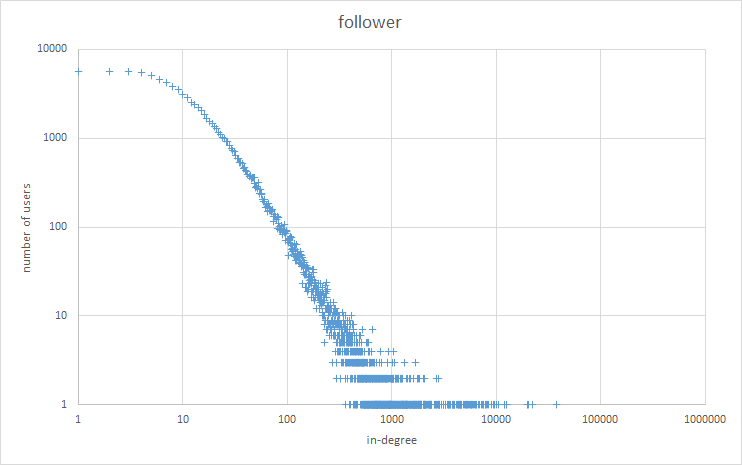
\includegraphics[width=\textwidth]{image13}
		\caption{follower graph}
	\end{subfigure}

	\caption{following 수와 follower 수에 따른 개발자의 수 분포 그래프. 가로 축과 세로 축 모두 log scale이다. 가로 축은 following/follower 수를 의미하고, 세로 축은 그러한 following/follower 수를 갖는 개발자의 수를 의미한다.}
	\label{fig:fdist}
\end{figure}


\subsection{개발자와 언어 사이의 관계}

\subsubsection{Multilingual 개발자 비율}

만약 모든 개발자가 한 가지 언어만 사용한다면, 개발자간의 관계에 의한 언어 전파는 발생하지 않는다고 할 수 있다. 그래서 가장 먼저 분석한 것은 여러 언어를 사용하는 개발자가 얼마나 되는가 하는 것이었다.

\begin{figure}
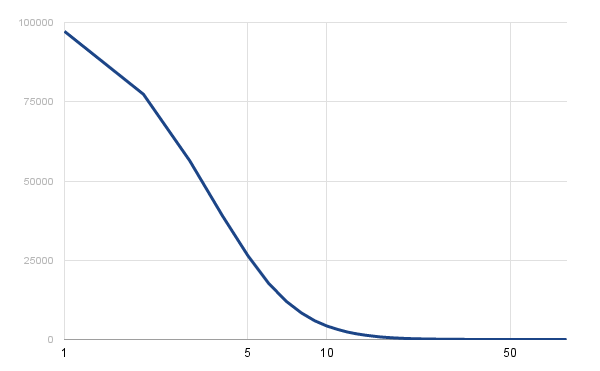
\includegraphics[width=\textwidth]{image10}
\caption{사용 언어 개수와 개발자 분포 그래프. 가로 축은 사용하는 언어의 수이고 세로 축은 그러한 개발자의 수를 나타낸다.}
\label{fig:langnum}
\end{figure}

한 가지 이상의 언어를 사용하는 97,206 명 중에서 2개 이상의 언어를 사용하는 사람은 77,355 명 존재했다. 즉, 여러 언어를 사용하는 개발자 비율이 0.796 이상이므로 다른 개발자에게 영향을 받아서 새로운 언어를 사용할 가능성도 충분히 있다고 볼 수 있다.

\subsubsection{언어별 Multilingual 개발자 비율}

\begin{figure}[ht]
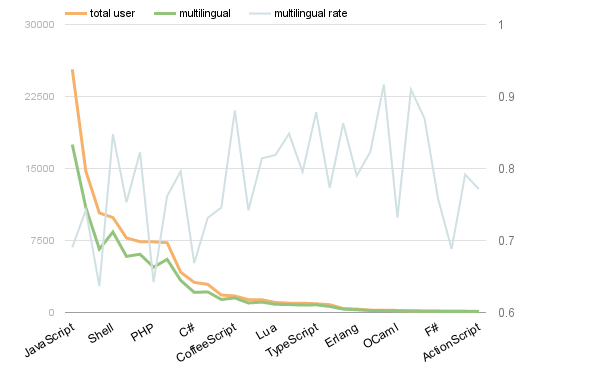
\includegraphics[width=\textwidth]{image04}
\caption{언어별 사용자수 및 multilingual 사용자수 그래프. 사용자수에 따라 정렬하였다.}
\label{fig:multilingual}
\end{figure}

\begin{longtable}{|c|r|r|r|}
\hline
\rowcolor[gray]{0.8}
언어 & total users & multilingual users & multilingual user rate \\
 \hline
 JavaScript & 25333 & 17494 & 0.690562 \\
 \hline
 Python & 14732 & 10932 & 0.742058 \\
 \hline
 Java & 10370 & 6602 & 0.636644 \\
 \hline
 Shell & 9889 & 8383 & 0.847710 \\
 \hline
 Ruby & 7765 & 5847 & 0.752994 \\
 \hline
 C & 7377 & 6068 & 0.822557 \\
 \hline
 PHP & 7358 & 4724 & 0.642022 \\
 \hline
 C++ & 7271 & 5537 & 0.761518 \\
 \hline
 Go & 4205 & 3348 & 0.796195 \\
 \hline
 C\# & 3135 & 2096 & 0.668581 \\
 \hline
 Objective-C & 2931 & 2144 & 0.731491 \\
 \hline
 Swift & 1821 & 1358 & 0.745744 \\
 \hline
 CoffeeScript & 1721 & 1516 & 0.880883 \\
 \hline
 Scala & 1337 & 992 & 0.741960 \\
 \hline
 Perl & 1329 & 1082 & 0.814146 \\
 \hline
 Lua & 1043 & 854 & 0.818792 \\
 \hline
 Rust & 976 & 828 & 0.848361 \\
 \hline
 Haskell & 967 & 769 & 0.795243 \\
 \hline
 TypeScript & 912 & 801 & 0.878289 \\
 \hline
 Clojure & 815 & 630 & 0.773006 \\
 \hline
 Groovy & 408 & 352 & 0.862745 \\
 \hline
 Erlang & 357 & 282 & 0.789916 \\
 \hline
 Kotlin & 249 & 205 & 0.823293 \\
 \hline
 Assembly & 228 & 209 & 0.916667 \\
 \hline
 OCaml & 220 & 161 & 0.731818 \\
 \hline
 Elm & 166 & 151 & 0.909639 \\
 \hline
 Scheme & 161 & 140 & 0.869565 \\
 \hline
 F\# & 157 & 119 & 0.757962 \\
 \hline
 Dart & 154 & 106 & 0.688312 \\
 \hline
 D & 144 & 114 & 0.791667 \\
 \hline
 ActionScript & 127 & 98 & 0.771654 \\
 \hline
\end{longtable}

개발자가 100명 이상인 언어 중에서 여러 언어를 사용하는 개발자의 비율은 위과 같다. 대체로 JavaScript, Java, C\#, PHP 등 전통적인 언어를 사용하는 개발자 중에서 여러 언어를 사용하는 개발자들의 비율이 작았다. 하지만 예외적으로 C++의 경우 다른 언어만큼 여러 언어를 사용하는 개발자가 있었고, C의 경우는 여러 언어를 사용하는 개발자의 비율이 높은 편이었다.

\subsection{언어간의 관계}

\subsubsection{Frequent Language Set}

\begin{longtable}{|l|l|}
\hline
\rowcolor[gray]{0.8}
Language set & \# of users \\
\hline

JavaScript, CSS, Python, HTML &
4415 \\ \hline
JavaScript, Python, Shell, HTML &
4039 \\ \hline
Ruby, JavaScript, Python, HTML &
3734 \\ \hline
Ruby, JavaScript, CSS, HTML &
3691 \\ \hline
Ruby, JavaScript, Python, Shell &
3590 \\ \hline
JavaScript, C, Python, HTML &
3531 \\ \hline
JavaScript, CSS, Shell, HTML &
3499 \\ \hline
JavaScript, Java, Python, HTML &
3453 \\ \hline
JavaScript, C, Python, Shell &
3445 \\ \hline

\end{longtable}

7개의 공통된 언어를 가지는 개발자 집합 중 가장 많은 수를 차지하는 집단은 Ruby, JavaScript, CSS, C, Python, Shell, HTML 을 사용하는 집단이었다. 그 외에도 많은 수를 차지하는 집단은 전부 JavaScript, CSS, HTML 을 사용하는 웹 프로그래머들이고, 서버 다른 서버 언어를 사용하는 집단이었다.


\subsubsection{Jaccard Distance}

\begin{center}
\begin{tabular} {|l|l|r|}
\hline
\rowcolor[gray]{0.8}
언어 1 & 언어 2 & Jaccard Distance \\
\hline

Python & 
Ruby & 
0.810189 \\ \hline
CSS & 
Ruby & 
0.810075 \\ \hline
CSS & 
Python & 
0.809257 \\ \hline
Java & 
JavaScript & 
0.802587 \\ \hline
HTML & 
Shell & 
0.801284 \\ \hline
C & 
Shell & 
0.800553 \\ \hline
HTML & 
Ruby & 
0.797200 \\ \hline
C++ & 
Python & 
0.794164 \\ \hline
JavaScript & 
Shell & 
0.770788 \\ \hline
Ruby & 
Shell & 
0.768404 \\ \hline
JavaScript & 
Ruby & 
0.767857 \\ \hline
C & 
Python & 
0.766779 \\ \hline
HTML & 
Python & 
0.766637 \\ \hline
Python & 
Shell & 
0.754458 \\ \hline
CSS & 
HTML & 
0.736205 \\ \hline
CSS & 
JavaScript & 
0.729116 \\ \hline
JavaScript & 
Python & 
0.722485 \\ \hline
C++ & 
C & 
0.718805 \\ \hline
Objective-C & 
Swift & 
0.716797 \\ \hline
HTML & 
JavaScript & 
0.684393 \\ \hline
\end{tabular}
\end{center}

또한, 각 언어 별 개발자 집합의 차이를 Jaccard Distance\cite{r11}를 이용해서 계산해보았다. Programming Language 중에서 가장 Jaccard Distance가 가까운 언어는 Objective-C와 Swift였다. Apple의 주력 언어가 Objective-C에서 Swift로 바뀌면서 옮겨간 사람들이 많은 것으로 보인다. 그 외의 웹 개발에 필수적인 JavaScript, CSS, HTML는 서로간의 Jaccard Distance가 가까운 것으로 나왔다.

만약에 서로 다른 성질을 가지는 언어 사이의 거리가 가까웠다면, 사람들은 필요에 의해서 새로운 언어를 배운다고 볼 수 있었을 것이다. 하지만 거리가 가까운 언어들은 대부분 비슷한 언어이거나, 비슷한 목적을 위한 언어였다. 따라서 어떤 언어의 기능이 부족하여 새로운 언어를 배운다는 가설은 틀렸다는 것을 알 수 있다.

\section{Closure Evolution}

D. Easley  2010 \cite{r2}에 의하면 소셜 네트워크에서 Affiliation Network를 구성하면, 관계가 형성되는 과정을 세 가지 관점에서 볼 수 있다. 두 사람 사이에 형성된 관계 사이에 공통된 이웃 사람이 있는 경우 triadic closure라고 하고, 두 사람 사이에 형성된 관계 사이에 공통된 foci가 있는 경우 focal closure라고 하고, 사람과 foci 사이에 형성된 관계 사이에 공통된 사람이 있는 경우 membership closure라고 한다. 관계가 형성되는 과정을 분석하기 때문에 시간에 따라 변하는 자료가 필요하다. 


\subsection{Triadic Closure}

공통된 이웃이 $k$명 있을 때 두 사람 사이에 관계가 형성되는 확률을 계산하였다. 관계 네트워크의 두 스냅샷이 있을 때, 다음과 같은 방식으로 계산하였다.
\begin{enumerate}
\item 먼저 모든 사람 쌍 사이의 공통된 이웃의 수를 계산하고, $k$마다 개수를 세어준다.
\item 새로 형성된 관계 사이에 기존에 공통된 이웃의 수가 몇 개였는지 세어준다.
\item 앞에서 계산한 개수들을 이용하여 새로 관계가 형성된 비율을 $k$에 따라 계산한다.
\end{enumerate}

$$
Pr(k) = \frac{\textrm{number of new links formed}}{\textrm{number of pairs that share } k \textrm{ neighbors}}
$$

다음은 계산 결과 표이다. $k$는 공통된 이웃의 수를 의미하고, $N_{pair}$는 공통된 이웃의 수가 $k$인 노드 쌍의 수를 나타낸다. 다음 snapshot 1→2와 2→3은 각각 스냅숏 1, 2, 3 사이에 새로 추가된 관계의 수를 의미한다. 이 수치를 이용해  공통된 이웃의 수가 $k$일 때, 스냅숏 사이에 관계가 생길 확률을 계산한 것이 $Pr(k)$이다. 다음 그래프는 스냅숏 사이에 관계가 생길 확률을 계산한 것을 그린 것이다. 단, 표본의 수가 너무 적은 경우 믿을 수 없는 값이 나오기 때문에 어느 정도 이상의 표본만 있는 $k$만 계산하였다. 새로 생긴 관계의 수가 약 20개 이상인 $k$에 대해서만 그래프에 나타내었다. 

\begin{longtable}{|c|r|r|r|l|}

\hline
\rowcolor[gray]{0.8}
$k$ & 
$N_{pair}$ & 
snapshot 1→2 &
snapshot 2→3 & 
$Pr(k)$ \\ \hline
0 & 
4228204249 & 
3834 &
3551 & 
0.00000087 \\ \hline
1 & 
839462339 & 
3478 &
3250 & 
0.00000401 \\ \hline
2 & 
314921931 & 
3160 &
2902 & 
0.00000962 \\ \hline
3 & 
121933392 & 
2299 &
2419 & 
0.00001934 \\ \hline
4 & 
49338414 & 
1654 &
1926 & 
0.00003618 \\ \hline
5 & 
22418306 & 
1167 &
1474 & 
0.00005850 \\ \hline
6 & 
11651207 & 
931 &
1144 & 
0.00008858 \\ \hline
7 & 
6741975 & 
637 &
959 & 
0.00011593 \\ \hline
8 & 
4218510 & 
548 &
782 & 
0.00015518 \\ \hline
9 & 
2793923 & 
430 &
601 & 
0.00018195 \\ \hline
10 & 
1936199 & 
361 &
596 & 
0.00023957 \\ \hline
11 & 
1394920 & 
264 &
394 & 
0.00023121 \\ \hline

$\cdots$ & 
$\cdots$ & 
$\cdots$ & 
$\cdots$ & 
$\cdots$  \\ \hline
\end{longtable}

\begin{figure}
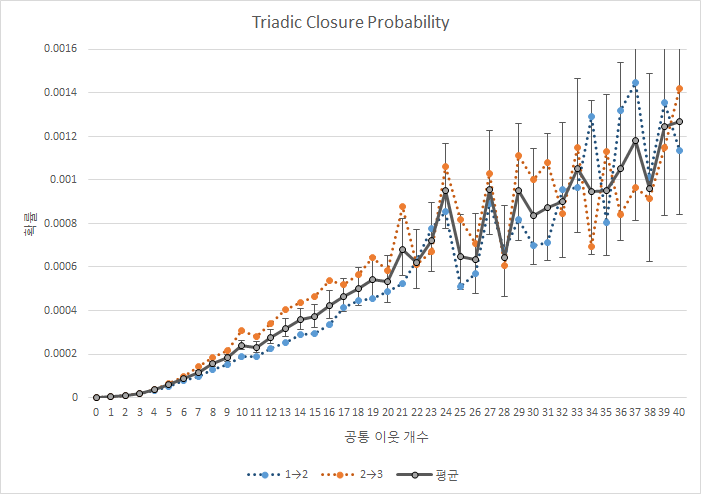
\includegraphics[width=\textwidth]{image14}
\caption{Triadic Closure 확률 그래프. 가로 축은 공통 이웃 개수를 의미하고, 세로 축은 링크가 형성될 확률을 의미한다. 파란색과 오렌지색은 snapshot 사이에서 계산한 것이고, 회색은 두 구간을 평균낸 것이다. Error bar도 표현하였다.}
\label{fig:triadic}
\end{figure}

관계가 생길 확률은 공통 이웃 개수에 대략 비례하는 것을 {\bf Figure \ref{fig:triadic}}의 그래프에서 확인할 수 있다. 공통 이웃 개수가 많아질수록 변동이 커지는 현상은 표본 수가 적어지면서 나타나는 현상이다.

Error bar는 Wilson score interval을 사용하여 계산하였다. Wilson score interval 공식은 다음과 같다\cite{r10}.

$$
\frac{1}{1 + \frac{1}{n}z^2} \left[ 
\hat{p} + \frac{1}{2n} z^2 \pm z 
\sqrt{\frac{1}{n} \hat{p} (1- \hat{p}) + \frac{1}{4n^2} z^2}
\right]
$$

생성되는 경우와 생성되지 않는 경우의 binomial distribution으로 보고 계산하였다. $z$ 값은 95\%에 해당하는 1.96을 사용하였다.


\subsection{Focal Closure}

foci가 있을 때, 공통된 foci의 개수에 따라 사람 사이의 관계가 형성될 확률을 분석하는 것이 focal closure 분석이다. foci는 두 가지로 정하고 분석하였다. Focus를 Language에 맞추어 계산한 경우와, Focus를 프로젝트에 맞추어 계산한 경우이다. Triadic Closure와 분석 방법은 별로 다르지 않다. 공통 이웃이 focus가 되도록 한 부분만 달라졌다.

\subsubsection{User vs Language}

Triadic Closure 계산할 때와 마찬가지 방법으로 계산할 수 있다. Focus는 사용 언어들이다. 다음 표와 
{\bf Figure \ref{fig:focallang}}의 
그래프는 계산 결과를 나타낸다.

$$
Pr(k) = \frac{\textrm{number of new links formed}}{\textrm{number of pairs that share } k \textrm{ languages}}
$$

\begin{longtable}{|c|r|r|r|l|}

\hline
\rowcolor[gray]{0.8}
$k$ & 
$N_{pair}$ & 
snapshot 1→2 &
snapshot 2→3 & 
$Pr(k)$ \\ \hline


0 &
3055384860 &
4989 &
4938 &
0.00000162 \\ \hline 
1 &
1665380554 &
7523 &
8032 &
0.00000467 \\ \hline 
2 &
586361957 &
4927 &
5456 &
0.00000884 \\ \hline 
3 &
194175745 &
1949 &
2490 &
0.00001135 \\ \hline 
4 &
66567753 &
1053 &
1178 &
0.00001673 \\ \hline 
5 &
24682353 &
465 &
594 &
0.00002129 \\ \hline 
6 &
9840528 &
238 &
306 &
0.00002742 \\ \hline 
7 &
4287003 &
123 &
171 &
0.00003383 \\ \hline 
8 &
1987914 &
57 &
102 &
0.00003836 \\ \hline 
9 &
982243 &
44 &
29 &
0.00003637 \\ \hline 
10 &
503983 &
21 &
24 &
0.00004455 \\ \hline 
11 &
265237 &
15 &
8 &
0.00004130 \\ \hline 

\end{longtable}

\begin{figure}
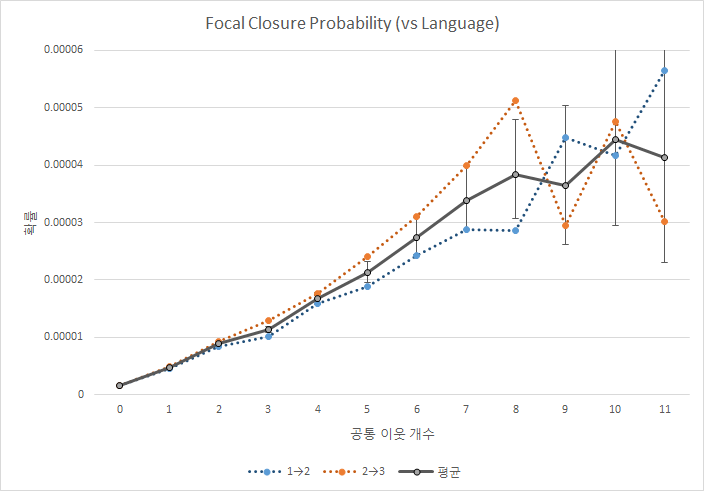
\includegraphics[width=\textwidth]{image16}
\caption{Focal Closure 확률 그래프. 가로 축은 공통 언어 개수를 의미하고, 세로 축은 링크가 형성될 확률을 의미한다. 파란색과 오렌지색은 snapshot 사이에서 계산한 것이고, 회색은 두 구간을 평균낸 것이다. Error bar도 표현하였다.}
\label{fig:focallang}
\end{figure}

Triadic Closure와 마찬가지로 공통 언어 개수가 많을수록 사용자끼리 관계를 맺을 가능성이 높았고 대략 비례하는 모습을 보였다. 마찬가지로 공통 이웃 개수가 많아질수록 새로 생긴 관계의 표본 수가 작아지면서 변동이 커지는 모습이 보였다.
error bar는 Wilson score interval을 사용하여 계산하였고 방법은 이전과 같다.



\subsubsection{User vs 프로젝트}

Focus를 언어 대신 프로젝트로도 계산해보았다. 마찬가지 방법으로 데이터를 얻었다. 다음 표와 {\bf Figure \ref{fig:focalrepo}}의 그래프는 프로젝트를 focus로 했을 때의 결과이다.

\begin{longtable}{|c|r|r|r|l|}

\hline
\rowcolor[gray]{0.8}
$k$ & 
$N_{pair}$ & 
snapshot 1→2 &
snapshot 2→3 & 
$Pr(k)$ \\ \hline
0 &
5579629872 &
19879 &
21348 &
0.00000369 \\ \hline
1 &
27268409 &
1103 &
1365 &
0.00004500 \\ \hline
2 &
2428933 &
265 &
329 &
0.00012156 \\ \hline
3 &
656830 &
62 &
154 &
0.00014877 \\ \hline
4 &
276701 &
46 &
58 &
0.00018667 \\ \hline
5 &
145173 &
10 &
16 &
0.00008713 \\ \hline
6 &
86001 &
19 &
22 &
0.00023773 \\ \hline
7 &
55999 &
6 &
12 &
 \\ \hline

\end{longtable}


\begin{figure}
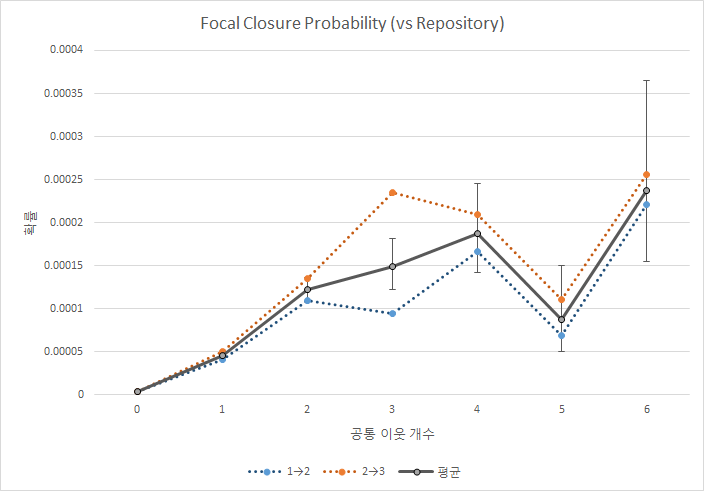
\includegraphics[width=\textwidth]{image07}
\caption{Focal Closure 확률 그래프. 가로 축은 공통 프로젝트 개수를 의미하고, 세로 축은 링크가 형성될 확률을 의미한다. 파란색과 오렌지색은 snapshot 사이에서 계산한 것이고, 회색은 두 구간을 평균낸 것이다. Error bar도 표현하였다.}
\label{fig:focalrepo}
\end{figure}

프로젝트는 언어에 비해 공유할 확률이 낮다. 그래서 대부분의 새로운 관계는 작은 $k$ 값에 더 집중이 되었다. 프로젝트 공통 개수가 7만 되어도 큰 의미가 없을 정도로 표본 수가 적어져서 6까지만 계산하였다. focus를 언어로 한 것에 비해 확실한 관계를 보기는 어려웠다.



\subsection{Membership Closure}


foci가 있을 때, 그 foci와 관계된 이웃 사람의 수에 따라 자신도 그 foci에 관계가 만들어질 확률을 분석한다. 이 경우에는 어떤 특정 언어를 사용하게 될 확률이 그 언어를 사용하는 이웃 개발자들의 수에 따라 어떻게 달라지는지 보는 것이다.
프로젝트와 관계되는 이벤트를 전부 알고 있기 때문에 스냅숏 방식을 사용하지 않고, 직접 계산할 수 있었다. 확률을 계산하기 위해서 다음과 같은 방식을 사용하였다. 먼저 다음 두 가지 경우의 수를 세어주었다.



$C_k$: 언어를 처음 사용했을 때, 이웃 사람 중 $k$명이 이미 사용하고 있었던 경우의 수

$D_k$: 결국 언어를 사용하지 않은 경우, 최종적으로 이웃 사람 중 $k$명이 언어를 사용하고 있는 경우의 수

그러면 언어를 사용하고 있는 이웃의 수 $k$에 따른 언어를 사용하게 될 확률은 다음과 같이 계산할 수 있다.


$$
Pr(k) = \frac{C_k}{\sum_{i=k}^{\infty}{C_i + D_i} }
$$

다음 {\bf Figure \ref{fig:infcurve}}의 그래프는 가장 인기 있는 프로그래밍 언어 네 개 Javascript, Python, Java, Ruby와 비교적 새로 등장한 언어인 Go와 Rust에 대해 그러한 확률을 분석한 결과를 그린 것이다. Rust는 자료가 부족하여 일부밖에 그릴 수 없었다.



\begin{figure}
	\begin{subfigure}{0.99\textwidth}
		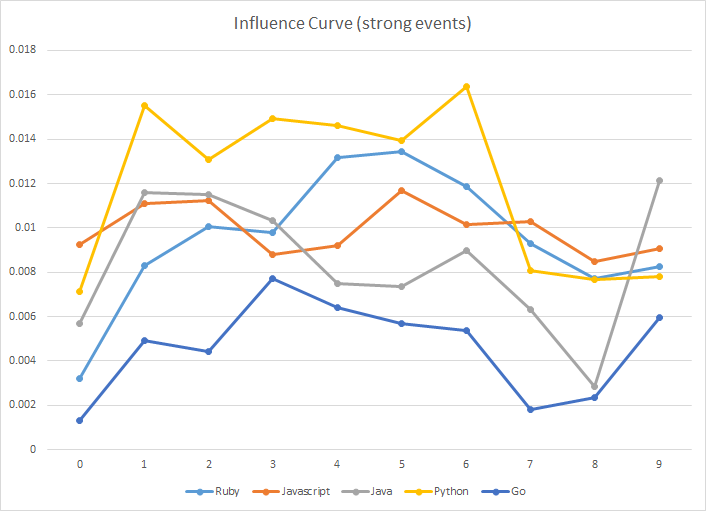
\includegraphics[width=\textwidth]{image01}
		\caption{Strong Events를 사용한 경우}
	\end{subfigure}

	\begin{subfigure}{0.99\textwidth}
		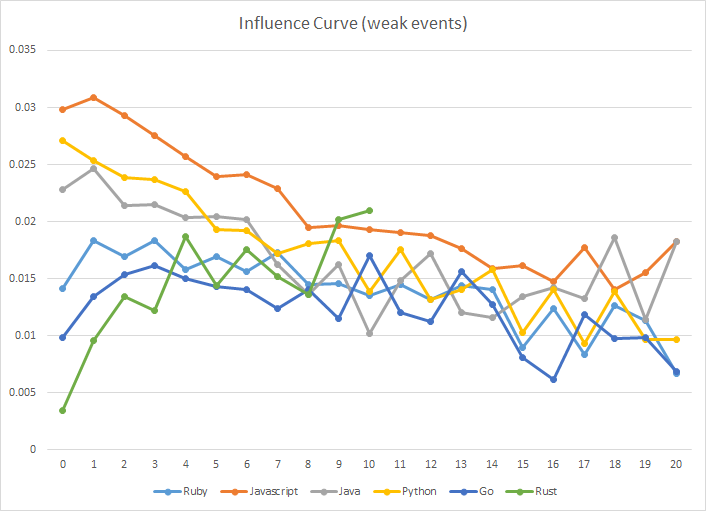
\includegraphics[width=\textwidth]{image18}
		\caption{Weak Events를 사용한 경우}
	\end{subfigure}

	\caption{특정 인원수의 주변인이 언어를 사용할 때 본인도 그 언어를 사용하게 될 확률을 나타낸 그래프이다.}
\label{fig:infcurve}
\end{figure}


Javascript와 Python은 피크가 0 또는 1에 있고 그 이후로 감소했다. Go나 Rust와 같이 비교적 새로 등장한 언어들은 피크가 비교적 늦게 나타나는 것을 볼 수 있었다. Go와 Rust의 경우 같은 언어를 사용하는 follow 관계에 있는 사람들이 많을수록 따라서 쓰는 경향이 더 강하다. 


\section{Language Propagation}

언어별로 개발자가 친구에게 영향을 받아 언어를 사용했는지 다른 이유로 사용했는지 알아보았다. 조사한 방법은 다음과 같다.
우선 GitHub Archive에 있는 최근 1년 4개월 동안의 Event 를 수집한다. Event에는 어떤 개발자가 어떤 프로젝트에 기여했는지 이분 그래프를 그릴 수 있다. 이를 다시 어떤 프로젝트가 어떤 언어를 사용하는지에 따라서 개발자 - 언어의 이분 그래프로 변환할 수 있다. 이를 이용하면 언어별로 개발자를 추출할 수 있다. 그 뒤, 특정 언어에 5번 이상 Event가 있는 개발자를 해당 언어의 개발자라고 보았다. 이 때, 이 개발자가 처음 Event를 발생시킨 시간을 이 사람이 처음 이 언어를 사용하기 시작한 시점으로 보았다.

이 자료를 가지고 언어를 사용한 순서대로 네트워크에 추가하며, follow 하는 사람을 edge로 연결 시켜 보았다. 그 결과 네트워크 내의 개발자 수와 독립된 그룹의 개수는 
{\bf Figure \ref{fig:cctrend}}과 같이 나왔다.

\begin{figure}
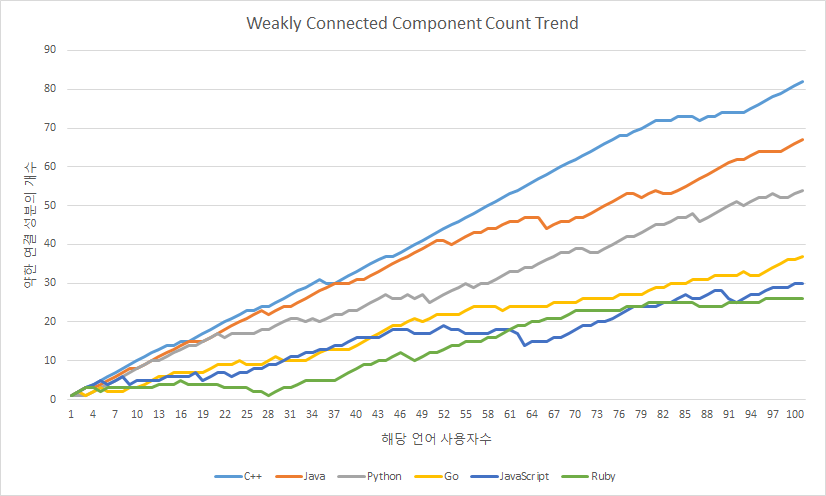
\includegraphics[width=\textwidth]{image11}
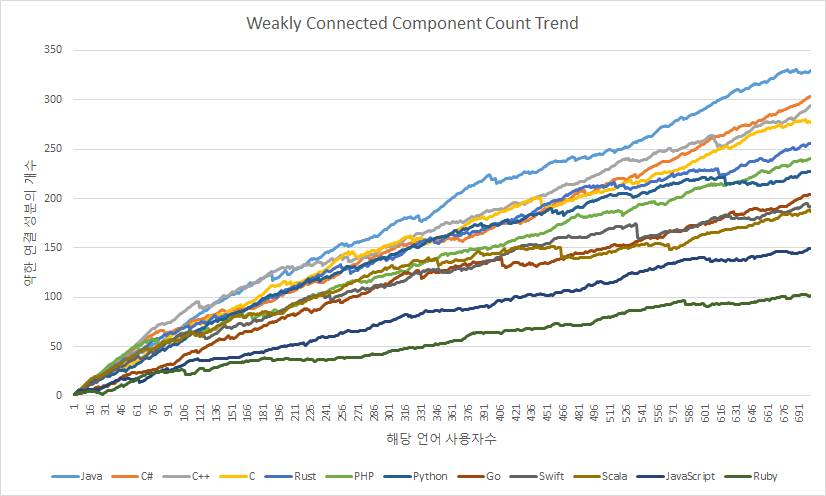
\includegraphics[width=\textwidth]{image_cc}
\caption{언어별 독립된 그룹의 개수 변화 그래프.}
\label{fig:cctrend}
\end{figure}

전체적으로 개발자 수가 늘어날수록 그룹의 수가 증가하는 것을 알 수 있다. 하지만 증가하는 정도는 언어에 따라서 다르다. 대표적으로 Java, C\#, C++, C의 경우 개발자 수가 증가하는 대로 그룹의 수가 빠르게 증가하는 것으로 나왔다. 이러한 언어들을 사용하기 시작하는 것에는 follow 관계가 영향을 적게 준다는 것을 알 수 있다. 이들은 전통적인 엔터프라이즈 시스템 개발에 많이 쓰이던 언어들이다. 이와 반대로 Ruby, JavaScript, Go 같은 언어는 개발자 수가 증가해도 그룹의 수가 잘 증가하지 않는다. 즉, 개발자 대부분이 follow 관계에 있다는 것을 알 수 있다. 이 언어들은 주로 스크립팅, 앱 개발, 또는 웹 개발 등에 많이 쓰이는 언어들이다. 이 언어들을 사용하는 사람들은 서로 follow 관계에 있을 가능성이 높다고 생각할 수 있다.


\section{Discussion}

이번 연구에서 우리는 GitHub 개발자의 소셜 네트워크와 프로그래밍 언어 사용 사이의 관계를 분석해 언어별 개발자 집단의 특성을 보고, 언어가 전파되는 과정에 있어 팔로우 관계를 통해 형성되는 지인 네트워크가 어떤 영향을 미치는지 살펴보았다.

GitHub을 이용하는 개발자 중에서 약 80\%는 2가지 이상의 언어를 사용하고 있다. 범위를 각 언어별로 한정했을 때도 대부분의 언어에서 70\% 이상의 사람은 해당 언어 외에 다른 언어 또한 사용하고 있다. 즉 이들은 처음 프로그래밍을 시작한 이후에 모종의 원인에 의해 새로운 언어를 추가적으로 습득한 사람들이다.

우리는 새로 습득한 언어가 기존에 사용하고 있던 언어와 어떤 관계가 있는지 알아보기 위해 각 언어 사이의 Jaccard Distance를 계산하여 보았다. 만약 사용하고 있는 언어의 기능이나 라이브러리, 성능 등이 마음에 들지 않아 새로운 언어를 사용하게 되는 것이라면, 차별화되는 기능을 제공하는 언어와의 거리가 가까울 것이다. 하지만 실제로는 그렇지 않았다. 서로의 거리가 가장 가까운 언어는 주로 웹 개발에 사용되는 JavaScript, HTML, CSS 였다. Objective-C와 Swift도 가까운 것으로 나타났으나, 두 언어는 애플 플랫폼의 주요 개발 언어가 바뀐 영향으로 볼 수 있어, 이 또한 기능의 차이 때문에 생긴 영향이 아니라 플랫폼 종속성에 의한 것으로 볼 수 있다. 즉, 새로 사용할 언어를 결정하는데 언어의 기능은 별로 중요한 것이 아니라는 것이다.

다음으로 주변의 지인이 특정 언어를 사용하는 것이 어떤 개발자가 새로운 언어를 습득하는 것에 영향을 주는지 여부를 확인하기 위해 기간을 두고 개발자의 follow 네트워크가 변하는 과정에서 세 가지 closure, 즉 triadic closure, focal closure, membership closure가 얼마나 영향을 끼치는지 계산해 보았다. 우선 triadic closure의 경우 연결돼 있지 않은 두 사람 사이에 공통된 친구가 많을수록 관계가 생길 확률이 높음을 확인할 수 있었다. focal closure에 대해서는 foci를 언어, 그리고 기여한 프로젝트 두 종류로 하여 각각의 closure 형성 여부를 확인하였다. 우선 언어를 foci로 해서 조사한 결과 연결돼 있지 않던 두 개발자 사이에 공통으로 사용하고 있는 언어가 많을 수록 새로 연결될 가능성이 높은 것으로 나타났다. 공동으로 기여한 프로젝트를 foci로 해 조사했을 땐 함께 기여하고 있는 프로젝트의 숫자가 많다고 해서 새로 관계가 형성될 확률이 높음을 확인하기 어려웠다. 이는 동시에 기여하는 프로젝트의 수가 많은 경우는 이미 관계가 형성돼 있기 때문일 확률이 높을 것으로 보인다. 마지막으로 membership closure, 즉 어떤 개발자가 아직 사용하고 있지 않은 언어를 이웃이 많이 사용할 경우, 새롭게 그 언어를 사용하게 될 지 여부를 조사해 보았다. 그 결과 언어별로 다른 양상을 보였는데, Javascript와 Python과 같이 이미 개발자층이 두텁고 역사가 오래된 언어에 비해 Go나 Rust처럼 비교적 최근에 인기를 얻은 언어의 경우 더 많은 이웃이 사용할 때 해당 언어를 사용하기 시작하는 것을 확인할 수 있었다.

또한, 언어를 사용한 순서대로 네트워크를 만들면서 네트워크 내의 독립된 그룹의 개수 변화를 관찰하였다. 여기서 C++, Java 등 전통적이고 산업에서 많이 사용되는 언어일수록 대부분의 개발자가 독립되어 있고, Ruby, JavaScript, Go 등의 언어는 대부분의 개발자가 연결되어 있음을 알 수 있다.


\section{Conclusion}

Membership Closure을 봤을 때, Go나 Rust같은 새로 생긴 언어들이 JavaScript나 Python같은 오래된 언어에 비해서 주변 개발자들이 사용할 때 언어를 사용할 확률이 높은 것으로 보였다.

language propagation을 봐도 비슷한 경향을 나타내는데, Java, C++, Python 등은 주변 사람들에게 큰 영향을 주지 못하지만, JavaScript, Ruby, Go 등의 언어는 언어를 사용하는 집단이 집단화 됐을 가능성이 높았다. 예외적으로 Rust의 경우 Membership Closure를 봤을 때, follow하고 있는 사이에서 전파될 확률이 높았지만, language propagation을 보면 영향을 덜 받는다고 나왔다. 이는 기존에 Rust를 쓰는 사람이 매우 적기 때문에 작은 변화에도 Membership closure가 크게 변했기 때문으로 보인다.

Triadic, Focal, Membership Closure를 계산하기 위해서는 시간에 따라서 변한 그래프가 필요하다. 하지만 GitHub은 팔로우 이벤트를 제공해주지 않기 때문에 우리는 최근 한 달 사이에 세 번의 스냅샷을 찍어 그래프를 만들 수밖에 없었다. 

수집한 정보로부터 네트워크가 진화하는 양상이나 언어가 퍼져나가는 양상은 분석할 수 있었다. 하지만 그러한 현상이 구체적으로 어떤 이유 때문에 일어나는 지까지는 알 수 없었다. 언어마다 다른 결과를 보이는 이유를 알아내거나 개발자들의 이용 패턴 등을 알아내기 위해서 실제 개발자들에게 설문을 돌리거나 다른 특성들을 추가로 조사해볼 수 있을 것이다.



\begin{thebibliography}{9}
\bibitem[1]{r1} GitHub, Where open source communities live, Retrieved from https://github.com/open-source 
\bibitem[2]{r2} D. Easley and J. Kleinberg, \emph{Networks, Crowds, and Markets: Reasoning About a Highly Connected World}, pp.95-97, July 2010.
\bibitem[3]{r3} L. A. Meyerovich and A. S. Rabkin, "Empirical analysis of programming language adoption," \emph{ACM SIGPLAN Notices}, Volume 48, Issue 10, pp. 1-18, 2013.
\bibitem[4]{r4} F. Thung, et al., "Network structure of social coding in github," \emph{Software maintenance and reengineering (csmr), 2013 17th european conference on}, IEEE, 2013.
\bibitem[5]{r5} Y. Yu, et al., "Exploring the patterns of social behavior in github," \emph{Proceedings of the 1st international workshop on crowd-based software development methods and technologies}, ACM, 2014.
\bibitem[6]{r6} A. Lima, L. Rossi, and M. Musolesi, "Coding together at scale: Github as a collaborative social network," \emph{CoRR}, abs/1407.2535, 2014.
\bibitem[7]{r7} GitHub, GitHub API v3 | Github Developer Guide, Retrieved from https://developer.github.com/v3/
\bibitem[8]{r8} GitHub Archive, Retrieved from https://www.githubarchive.org/
\bibitem[9]{r9} GitHub, Events | GitHub Developer Guide, Retrieved from https://developer.github.com/v3/activity/events/
\bibitem[10]{r10} E. B. Wilson, "Probable inference, the law of succession, and statistical inference," \emph{Journal of the American Statistical Association}, Volume 22, No. 158, pp. 209-212, 1927.
\bibitem[11]{r11} M. Levandowsky and D. Winter, "Distance between sets," \emph{Nature}, 234(5), pp. 34-35, doi:10.1038/234034a0, 1971.

\end{thebibliography}

\end{document}

